\section{Run on the same node of RNN-MSNN with different batch
size}\label{run-on-the-same-node-of-rnn-msnn-with-different-batch-size}

Test report

by E. Marquer, 2018/06/15 Synalp and Université de Lorraine

\subsection{Abstract}\label{abstract}

The test is composed of 2 runs: - id 1583339: batch-size 1, bptt 200 on
grele-2 - id 1583336: batch-size 2, bptt 100 on grele-1

Run time per epoch varies from 28 to 20 min for a single batch and from
20 to 11 min for two batches.

\subsubsection{Shared parameters}\label{shared-parameters}

\begin{longtable}[]{@{}ll@{}}
\toprule
parameter & value\tabularnewline
\midrule
\endhead
corpus & enwik8reduced\tabularnewline
history\_strategy & layer-constant-length\tabularnewline
max\_history & 25\tabularnewline
bptt & \emph{variable}\tabularnewline
batch\_size & \emph{variable}\tabularnewline
epochs & 4\tabularnewline
lr & 1e-3\tabularnewline
weight\_decay & 1.2e-6\tabularnewline
epochs & 4\tabularnewline
valid\_len & 500,000\tabularnewline
log\_interval & 500\tabularnewline
save\_interval & 500\tabularnewline
memory\_interval & 100\tabularnewline
hidden\_size & 460\tabularnewline
embed\_size & 400\tabularnewline
growth\_factor & 5\tabularnewline
rnn\_type & RNN\tabularnewline
reset\_hidden & False\tabularnewline
reset\_growth & True\tabularnewline
cuda\_on & True\tabularnewline
\bottomrule
\end{longtable}

\subsection{Results}\label{results}

At the end of each epoch, we see a spike in BPC, due to the first
evaluation of the epoch (BPC is reinitialised to 0, causing a spike).
With 2 btches, BPC is also more stable.

As of now, run time is computed after running validation, so training
time is \lstinline!real_training_time = run_time - validation_time!. But
validation time increase with the number of batches as the number of
characters seen increase (the whole validation corpus is used for each
batch, so the number of characters seen during validation is
\lstinline!validation_corpus_len * batches!). That explains that the
evaluation time for a batch is lower than for 2 batches.

By removing evaluation time, we can obtain a reasonable and coherent
(with regard to epoch run time) estimation of training time over a
sequence.

\subsubsection{Epoch run time:}\label{epoch-run-time}

\begin{longtable}[]{@{}lll@{}}
\toprule
Epoch & Run time b=1 & Run time b=2\tabularnewline
\midrule
\endhead
1 & 28 min & 20 min\tabularnewline
2 & 23 min & 17 min\tabularnewline
3 & 22 min & 14 min\tabularnewline
4 & 20 min & 11 min\tabularnewline
\bottomrule
\end{longtable}

There is a notable decrease in epoch run time (time necessary to run
over an epoch), of about 10 min over the 4 epochs, with both runs.

Possible causes for the decrease of run time: - part of the graph is
already computed, and this part is skipped; - corpus data is already
loaded in cuda memory.

Both of them are highly unlikely to cause such a decrease. A more
precise training time storage may provide an explanation.

\subsubsection{Plots}\label{plots}

\begin{figure}
\centering
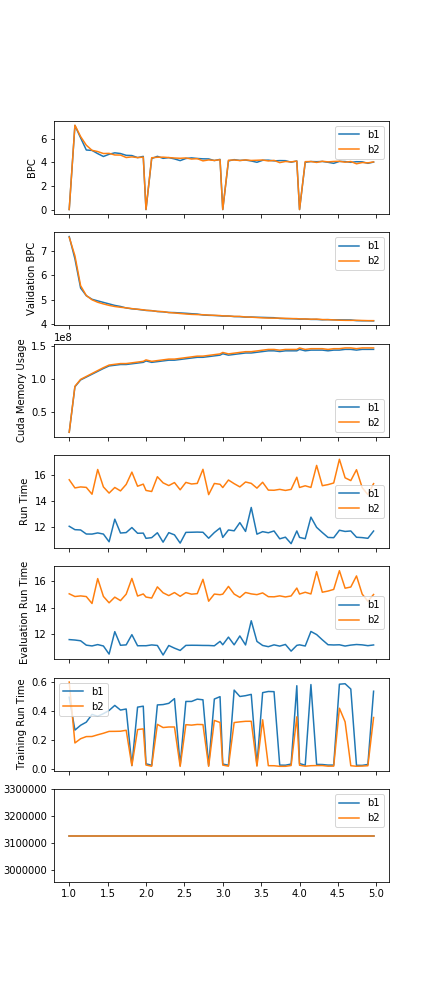
\includegraphics{2018_06_15_frac.png}
\caption{Full data}
\end{figure}

\begin{figure}
\centering
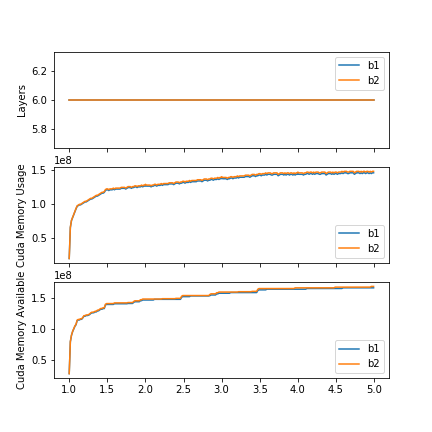
\includegraphics{2018_06_15_memory.png}
\caption{Memory usage}
\end{figure}

\subsection{Next steps}\label{next-steps}

\begin{itemize}
\tightlist
\item
  Data

  \begin{itemize}
  \tightlist
  \item
    Implement more precise time data saving (epoch run time and training
    run time)
  \end{itemize}
\item
  Runs (objective: 100 epochs)

  \begin{itemize}
  \tightlist
  \item
    Continue running batches 1 and 2
  \item
    Try with higher number of batches
  \end{itemize}
\item
  {[}Optional{]} Other experimental branch

  \begin{enumerate}
  \def\labelenumi{\arabic{enumi}.}
  \tightlist
  \item
    Implement prepared attention module in every layer
  \item
    Analyse results
  \item
    Patch probable memory leaks
  \end{enumerate}
\end{itemize}
